\documentclass{article}
\usepackage[T1]{fontenc}
\usepackage[utf8]{inputenc}
\usepackage{microtype}
\usepackage{graphicx}
\usepackage{booktabs}
\usepackage{multirow}
\usepackage{hyperref}
\usepackage{icml2026}
\usepackage{amsmath,amssymb}
\graphicspath{{figures/}}
\newcommand{\Sig}{\Sigma}
\newcommand{\Lz}{L_0}
\icmltitlerunning{Sparse Autoencoder Decoder Spectra Against a Covariance-Matched Null}
\begin{document}
\twocolumn[
  \icmltitle{Sparse Autoencoder Decoder Spectra Against a Covariance-Matched Null}
  \begin{icmlauthorlist}
    \icmlauthor{Anonymous Authors}{anon}
  \end{icmlauthorlist}
  \icmlaffiliation{anon}{Anonymous Institution}
  \icmlcorrespondingauthor{Anonymous Authors}{anon@example.org}
  \icmlkeywords{sparse autoencoders, interpretability}
  \vskip 0.3in
]
\printAffiliationsAndNotice{}
\begin{abstract}
The decoder directions of a sparse autoencoder (SAE) form a point cloud whose covariance eigenvalues fall as a power law, and the slope of that power law has been read as a property of the model layer the SAE was trained on. We argue that the slope can only be read against a fixed sparsity and a matched null, and that against a Gaussian with the activations' mean and covariance $\Sig$, real activations show up most clearly in the bulk of the decoder spectrum and in its profile across layers. On 28 Gemma Scope SAEs at one layer of Gemma-2-2B, the slope over ranks 11--150 rises by $0.099$ per doubling of the number of active latents $\Lz$, so we compare TopK SAEs trained on real and on Gaussian data at the same $k=40$. At layers 3, 13 and 23, ranks 31--1000 of the real spectrum are 2.1 to 4.7 times flatter than the null's in every cell. Relative to the null, the real top ranks are steepest at layer 13. In the top 150 ranks the two give slopes of the same order, but they agree closely only at some $k$ and some layers. A TopK SAE cannot code the Gaussian sparsely (fraction of variance unexplained 0.53--0.60, against 0.18--0.29 on real data). These comparisons therefore separate real activations from a dense covariance-matched null, not from a sparse one.
\end{abstract}


\section{Introduction}

\citet{li2025geometry} found that the decoder directions of Gemma Scope SAEs \citep{lieberum2024gemmascope} have a power-law covariance spectrum that is steepest in the middle of the network. Their layer-12 slope ($-0.47$) has become a reference number for the geometry of SAE features, and a replication on TopK SAEs found slopes of $-0.54$ to $-0.72$ \citep{peter2025progressive}. This paper asks which parts of that spectrum depend on the activations beyond their second moments. We find that any answer depends on two things: the operating point, because the slope moves with sparsity, and the null, because an SAE produces a power-law spectrum from an anisotropic covariance alone. Against a dense Gaussian null at fixed sparsity, the real spectrum differs most in its bulk and in its profile across layers. The top-window slope, which is the number usually reported, differs less and in a way that depends on $k$.

The null is the same TopK SAE \citep{gao2024scaling} trained on samples from $N(\mu,\Sig)$, with $\mu$ and $\Sig$ estimated from the real activations. A second null permutes each coordinate independently across tokens, which keeps every marginal distribution and removes all correlations. A random rotation would not serve as a null, because the spectrum is rotation-invariant. The Gaussian null keeps what an SAE could learn from second moments, but it also removes sparse codability. Real activations are reconstructed from 40 active latents with a fraction of variance unexplained (FVU) of 0.18--0.29, and Gaussian samples with 0.53--0.60. A difference between the two SAEs therefore reflects everything the Gaussian lacks, sparsity included. A null that keeps sparse codes and matches $\Sig$ is the comparison that would isolate structure beyond ``sparse plus $\Sig$''. It is not part of the present evidence.
%% PENDING-GPU: sparse covariance-matched null (layer-13 k sweep and 8 layers). When it lands, this paragraph states whether bulk and profile differences survive a null that is sparsely codable; the abstract's last sentence changes accordingly.

The comparison needs a fixed operating point, because the decoder slope is not a fixed property of a layer. Across 28 Gemma Scope SAEs at layer 12 the slope runs from $-0.73$ at $\Lz \approx 12$ to $-0.24$ at $\Lz \approx 444$. The height of the mid-stack peak falls from 0.23 to 0.06 between $\Lz=40$ and $\Lz=140$. We therefore compare real and null SAEs at the same $k$, and report four rank windows throughout.

\textbf{Contributions.}
(1)~The decoder slope at fixed layer rises by $0.099$ per doubling of $\Lz$, and the mid-stack peak shrinks with $\Lz$ (Section~\ref{sec:l0}).
(2)~At layers 3, 13 and 23 of Gemma-2-2B and $k=40$, real and Gaussian-null SAEs differ consistently in the bulk of the spectrum and in the layer profile of the top ranks. We report FVU beside each comparison, and one pair of runs matched in FVU (Section~\ref{sec:null}).
(3)~Null decoders do not collapse onto near-duplicate latents. Gaussian-null decoders are closer than real decoders to a power of $\Sig$ along $\Sig$'s own axes, with a much larger exponent in the bulk, and scrambled-null decoders follow the axes of their own covariance $\mathrm{diag}(\Sig)$ (Section~\ref{sec:regime}).
(4)~A sparse dictionary that matches only the second moments of Gemma Scope's directions reproduces the drop of $\gamma$ between $k=8$ and 16 but not all of the steady decline above it. Over the pre-registered $k=8$--128 it retains 0.78 of the decline in ranks 11--150 and 0.53--0.62 in the bulk, over three draws and two seeds; over $k=16$--128, chosen post hoc, 0.45 (Section~\ref{sec:k}).
(5)~We reconcile \citet{li2025geometry}'s statement that activation spectra decay more slowly than decoder spectra. The raw activation covariance is steeper than the decoder at all 26 layers. After per-dimension standardisation their ordering holds at 4 to 9 middle layers (Section~\ref{sec:setup}).

\section{Related work}

\textbf{SAE decoder geometry.} \citet{li2025geometry} reported the power law, its mid-stack peak, and cluster structure in Gemma Scope decoders, and left the origin of the power law open. \citet{peter2025progressive} replicated the power law on three TopK SAEs and found that larger SAEs decay slightly less steeply. Their larger SAEs also had larger $k$, so width and sparsity are confounded there; Section~\ref{sec:l0} separates them. \citet{borobia2026nearfloor} compare a geometric property of trained decoders with a matched i.i.d.\ control and count only the excess, the same design we use for a different statistic.

\textbf{Nulls for SAEs.} SAEs trained on randomly initialised transformers score like trained ones on several interpretability metrics \citep{heap2025random}, and frozen random components match trained SAEs on probing and editing \citep{korznikov2026sanity}. Those nulls randomise the model. Ours keeps the model and randomises the data beyond its second moments. \citet{engels2025darkmatter} show that much SAE error is linearly predictable from the input.

\textbf{Data statistics and learned geometry.} Representation spectra are anisotropic \citep{ethayarajh2019contextual} and often follow power laws \citep{ghosh2022powerlaws}. In toy models, feature correlations shape the geometry of superposition \citep{prieto2026correlations}. \citet{saraswatula2025whitening} argue that SAEs trained on unwhitened inputs are biased toward high-variance directions and show that whitening improves interpretability metrics. They do not measure decoder spectra. A whitened-input SAE would test directly how much of the spectrum $\Sig$ sets. We have not run it.

\textbf{Allocation theories.} \citet{michaud2025manifolds}, adapting \citet{brill2024scaling}, model how SAE latents are allocated to features of different frequencies and derive an exponent for the number of latents per feature. They make no prediction about decoder spectra. Turning their exponent into a spectral slope needs an extra assumption, which is ours (Appendix~\ref{app:fail}). Feature splitting and absorption \citep{chanin2025absorption}, dense latents \citep{sun2025dense} and massive activations \citep{sun2024massive} are other candidate sources of decoder anisotropy.

\section{Setup and definitions}
\label{sec:setup}

\textbf{Decoder spectrum.} An SAE with $n$ latents has unit-norm decoder rows $w_1,\dots,w_n \in \mathbb{R}^d$ ($d=2{,}304$ for Gemma-2-2B). We sort the eigenvalues $\lambda_1 \ge \lambda_2 \ge \dots$ of the rows' centred covariance. The \emph{eigen-slope} over a rank window $[a,b]$ is the least-squares slope of $\log_{10}\lambda_r$ on $\log_{10} r$ for $a \le r \le b$. A more negative slope means a more anisotropic cloud. For Gemma Scope SAEs we use all rows, as \citet{li2025geometry} do. For our own TopK SAEs we use the rows of latents that fire at least once on held-out tokens. On 22 layer-12 Gemma Scope SAEs with up to 13.9\% dead rows, the two conventions differ by at most 0.003 in ranks 11--150 and 0.013 in ranks 101--1000. TopK SAEs are more sensitive. On local layer-12 TopK SAEs trained on PCA projections of the activations (width 8,192, $k=8$), with 11\% of rows dead the two differ by 0.025 in ranks 11--150, and with 33--42\% dead by up to 0.09 in ranks 11--150 and 0.22 in ranks 101--1000. Our $k=40$ SAEs have at most 2.4\% of rows dead (Table~\ref{tab:fvu}). In the $k$ sweep of Section~\ref{sec:k}, 11--12\% of rows are dead at $k=16$ in both conditions and at $k=8$ in the Gaussian null. In the real SAEs at $k \le 8$ 60--96\% are dead, and in the null at $k \le 4$ 90--97\%. Values in those runs are live-row values that are not comparable with all-row slopes, and we mark them where we use them.

\textbf{Rank windows.} The spectrum is curved, so the slope depends on the window. Before the experiments we fixed four windows. Ranks 4--50 and 11--150 are the \emph{top windows}, with 11--150 primary; ranks 31--450 and 101--1000 are the \emph{bulk windows}. A conclusion was to count only if it held in the primary window and at least two others. The windows overlap, and ranks 11--150 contain 40 of the 47 ranks in 4--50.

\textbf{Activation covariance and $\gamma$.} $\Sig$ is the centred covariance of residual-stream activations (\texttt{resid\_post}). For Gemma Scope SAEs we estimate it from 1,002,540 Pile tokens. For our own SAEs we estimate it from their 10M training tokens. The relative exponent is $\gamma = s_{\mathrm{dec}}/s_{\Sig}$, the decoder eigen-slope divided by $\Sig$'s slope in the same window. A value of $\gamma<1$ means the decoder spectrum falls less steeply than $\Sig$'s. Within one layer $\gamma$ is the slope divided by a constant, so it is useful only across layers or inputs whose $\Sig$ differ. Real and Gaussian-null SAEs share $\Sig$, so for them we report raw slopes.

\textbf{Activation and decoder spectra.} \citet{li2025geometry} state that activation spectra decay much more slowly than SAE-feature spectra, which would mean $\gamma>1$. Their exponent for the decoder is fitted over ranks 11--150. Their activation-to-feature comparison uses the 100 largest eigenvalues. Their protocol for the activations is not given, so we varied it at layer 12 against their SAE (width 65k, $\Lz=72$ by release name, 75.8 measured on our tokens), whose decoder slope over ranks 1--100 is $-0.462$. The raw centred covariance gives $-0.923$, and unit-normalised tokens, uncentred activations and the SAE's own codes give $-0.88$ to $-1.03$. Standardising each dimension gives $-0.446$, slightly flatter than the decoder. On the 1M-token covariance at all 26 layers, the raw activation spectrum is steeper than the decoder at 26 of 26 layers. After standardisation, Li et al.'s ordering holds at 4 layers (11--14) against their SAEs and at 9 layers (10--18) against 16k SAEs at $\Lz \approx 40$ (Appendix~\ref{app:li}). Their remark is therefore consistent with standardised mid-stack activations and not with the raw covariance. We use the raw centred covariance throughout.
%% PENDING-GPU: Gemma-2-9b out-of-sample predictions (Li et al.'s model). When they land, add one sentence here on whether the raw/standardised ordering carries over to Gemma-2-9b.

\textbf{Sparsity and live latents.} $\Lz$ is the mean number of active latents per token; for TopK SAEs $\Lz=k$. For Gemma Scope JumpReLU SAEs \citep{rajamanoharan2024jumprelu} we measured $\Lz$ on 1M tokens where we had the encoder (22 of the 28 layer-12 SAEs) and otherwise took it from the release name. Finite clouds bias $\gamma$. An isotropic cloud of 16,384 unit vectors in $d=2{,}304$ measures $\gamma=0.054$ in ranks 11--150. A Gaussian cloud whose true exponent is 1 measures 0.741 at 672 points and 0.974 at 16,384 (Appendix~\ref{app:live}). We compare conditions where their live counts are similar and say so where they are not.

\textbf{SAEs.} We analyse the decoders of 288 Gemma Scope residual-stream SAEs (widths 16k to 1M). Our own SAEs are TopK with an auxiliary loss for dead latents \citep{gao2024scaling}. We trained them on Gemma-2-2B layers 3, 13 and 23 at widths 16,384 and 65,536 with $k=40$, three seeds per cell, on real activations and on both nulls (54 SAEs). Each run makes three passes over about 9.5M Pile tokens and is evaluated on 0.5M held-out tokens. A $k$ sweep at layer 13, width 16,384, covers $k \in \{1,2,4,8,16,40,128\}$ with two seeds, real and Gaussian. Appendix~\ref{app:methods} gives hyperparameters and window indexing.

\section{The decoder slope moves with $\Lz$}
\label{sec:l0}

\begin{figure*}[t]
\centering
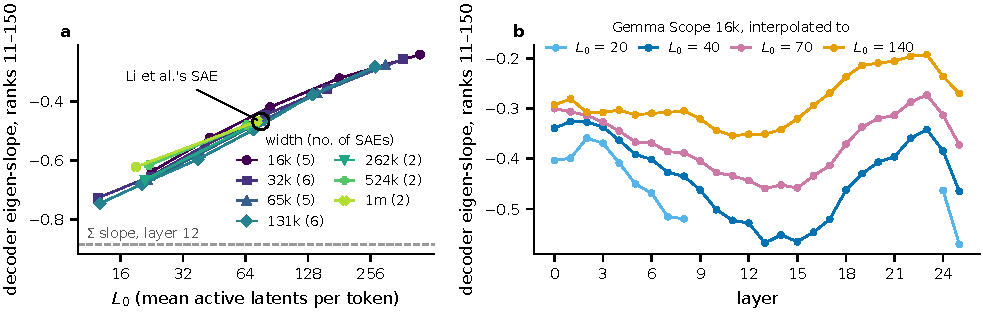
\includegraphics[width=\textwidth]{thesisA_fig1_setup.pdf}
\caption{At a fixed layer the decoder slope moves with sparsity. (a) Layer 12, 28 Gemma Scope SAEs at seven widths, all decoder rows. The slope in ranks 11--150 rises by $0.099$ per doubling of $\Lz$, from $-0.73$ at $\Lz=12$ to $-0.24$ at $\Lz=444$. \citeauthor{li2025geometry}'s SAE ($-0.468$, circled) lies on the line. The dashed line is $\Sig$'s slope (1M tokens). (b) Gemma Scope 16k decoders interpolated to fixed $\Lz$ across the 26 layers. The mid-stack peak is 0.23 below layer 0 at $\Lz=40$ and 0.06 at $\Lz=140$. Gaps mark layers whose SAEs do not bracket $\Lz=20$.}
\label{fig:l0}
\end{figure*}

At one layer, sparsity sets much of the decoder slope (Figure~\ref{fig:l0}a). Across the 28 layer-12 Gemma Scope SAEs, the slope in ranks 11--150 is linear in $\log_2 \Lz$ with slope $0.099$ per doubling ($R^2=0.984$), from $-0.727$ at $\Lz=12$ to $-0.242$ at $\Lz=444$. At matched $\Lz$ (19--24, 36--44 and 64--86) SAEs of different width differ by 0.063, 0.073 and 0.076. That is about two-thirds of the effect of one doubling of $\Lz$ and small against the 0.49 range over the 37-fold range of $\Lz$. The SAEs at widths 524k and 1M near $\Lz=20$ lie visibly above the line. \citet{li2025geometry}'s $-0.468$ belongs to the 65k SAE at $\Lz=72$. \citet{peter2025progressive}'s larger SAEs were also less sparse, which fits their finding that larger SAEs are flatter.

The layer profile depends on $\Lz$ too (Figure~\ref{fig:l0}b). With the 16k Gemma Scope SAEs interpolated to fixed $\Lz$, the steepest layer in ranks 11--150 is 13 at $\Lz=40$ and 70. The peak sits 0.23 below layer 0 at $\Lz=40$, 0.16 at $\Lz=70$ and 0.06 at $\Lz=140$. The rank window matters on a similar scale. Li et al.'s SAE has slopes $-0.476$, $-0.468$, $-0.418$ and $-0.503$ in our four windows.

Across layers the decoder profile follows $\Sig$'s. $\Sig$'s slope in ranks 11--150 is steepest at layer 13 ($-0.944$, against $-0.726$ at layer 0). At $\Lz=40$ the Gemma Scope 16k decoder slope correlates with it across the 26 layers at Pearson $r=0.92$. Adjacent layers are not independent. Bartlett's effective sample size is 6.5, which gives a 95\% interval of $[0.50, 0.99]$. Phase-randomised surrogates give $p<10^{-4}$, and circular shifts give $p=0.038$, the smallest value that 26 shifts can produce. Over the top windows at $\Lz=40$ and 70 and both widths, $r=0.75$--$0.92$ with effective sizes 6.4--7.0. The intervals' lower ends run from $-0.01$ to 0.50, so one of them includes zero, and phase-surrogate $p \le 0.024$. In ranks 31--450 at $\Lz=40$ the correlation is $r=0.81$ (16k) and 0.76 (65k), with phase-surrogate $p=0.021$ and 0.037, so at $\Lz=40$ it holds in the primary window and two others. At $\Lz=70$ the same window gives $p=0.051$ and 0.058. In ranks 101--1000 the surrogate $p$ is 0.068--0.127 at $\Lz=40$ and 70. At $\Lz=140$ there is no detectable correlation in the top windows ($r=0.37$ in ranks 11--150, phase-surrogate $p=0.60$). The correlation is observational. The objective could pass $\Sig$'s shape to the decoder, or $\Sig$ and the decoder could both reflect depth-dependent structure in the activations. Section~\ref{sec:profile} tests the first reading.

\section{Real activations against covariance-only SAEs}
\label{sec:null}

\begin{table*}[t]
\centering
\caption{Decoder eigen-slope of our TopK SAEs at $k=40$, width 16,384, mean of three seeds (largest seed sd 0.013), live rows. $\Sig$ is estimated from the 10M training tokens; the scrambled null's own covariance is $\mathrm{diag}(\Sig)$. FVU and live counts are in Table~\ref{tab:fvu}; width 65,536 is in Table~\ref{tab:65k}. Bold marks the steepest layer for the real SAE in each top window.}
\label{tab:null}
\small
\setlength{\tabcolsep}{3.6pt}
\begin{tabular}{l rrr rrr rrr rrr}
\toprule
 & \multicolumn{3}{c}{ranks 4--50} & \multicolumn{3}{c}{ranks 11--150} & \multicolumn{3}{c}{ranks 31--450} & \multicolumn{3}{c}{ranks 101--1000} \\
\cmidrule(lr){2-4}\cmidrule(lr){5-7}\cmidrule(lr){8-10}\cmidrule(lr){11-13}
layer & 3 & 13 & 23 & 3 & 13 & 23 & 3 & 13 & 23 & 3 & 13 & 23 \\
\midrule
SAE on real & $-0.224$ & $\mathbf{-0.475}$ & $-0.340$ & $-0.290$ & $\mathbf{-0.481}$ & $-0.292$ & $-0.554$ & $-0.446$ & $-0.280$ & $-0.676$ & $-0.571$ & $-0.389$ \\
SAE on $N(\mu,\Sig)$ & $-0.255$ & $-0.276$ & $-0.286$ & $-0.424$ & $-0.505$ & $-0.507$ & $-1.181$ & $-1.050$ & $-0.972$ & $-2.394$ & $-1.921$ & $-1.841$ \\
SAE on scrambled & $-0.226$ & $-0.391$ & $-0.427$ & $-0.349$ & $-0.649$ & $-0.976$ & $-1.357$ & $-0.954$ & $-0.761$ & $-2.315$ & $-1.241$ & $-0.341$ \\
\midrule
$\Sig$ (10M tokens) & $-0.714$ & $-0.982$ & $-0.807$ & $-0.676$ & $-0.947$ & $-0.749$ & $-0.846$ & $-0.750$ & $-0.697$ & $-0.961$ & $-0.705$ & $-0.679$ \\
\bottomrule
\end{tabular}
%% PENDING-GPU: real vs Gaussian at 8 layers with 3 seeds. Extend this table (or add Table rows) to the 8 layers; the layer-profile statements in Sec. 5.3 and the abstract are rewritten from that table.
\end{table*}

\begin{table}[t]
\centering
\caption{Regime of the $k=40$ SAEs: eval FVU (mean of three seeds; seed range $\le 0.003$) and live latents (range over seeds, of 16,384 or 65,536).}
\label{tab:fvu}
\footnotesize
\setlength{\tabcolsep}{2.5pt}
\begin{tabular}{ll rrr}
\toprule
width & condition & layer 3 & layer 13 & layer 23 \\
\midrule
\multirow{3}{*}{16k} & real & 0.204 & 0.288 & 0.287 \\
 & Gaussian & 0.565 & 0.528 & 0.603 \\
 & scrambled & 0.642 & 0.614 & 0.766 \\
\multirow{3}{*}{65k} & real & 0.178 & 0.290 & 0.276 \\
 & Gaussian & 0.559 & 0.526 & 0.594 \\
 & scrambled & 0.636 & 0.610 & 0.747 \\
\midrule
16k live & real & 16.38k & 16.24--16.28k & 16.37--16.38k \\
65k live & real & 65.37--65.41k & 63.97--64.34k & 65.24--65.34k \\
\multicolumn{2}{l}{both nulls, both widths} & \multicolumn{3}{c}{all live except $\le 2$ rows} \\
\bottomrule
\end{tabular}
\end{table}

\begin{figure*}[t]
\centering
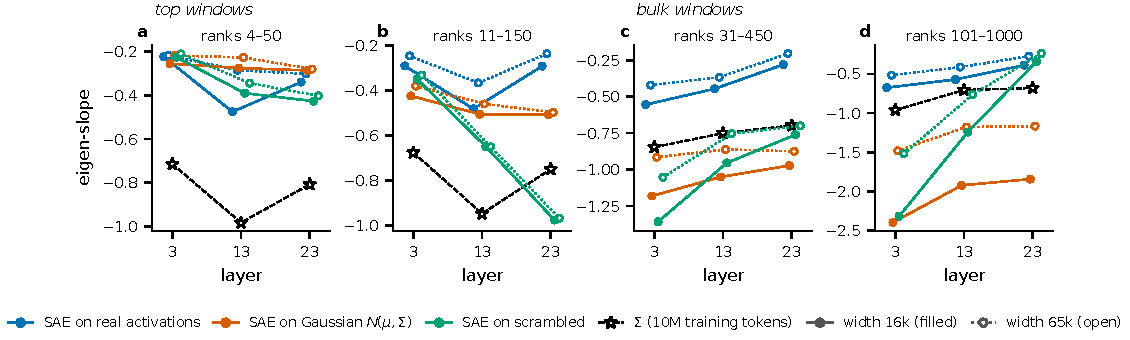
\includegraphics[width=\textwidth]{thesisA_fig2_null_layers.pdf}
\caption{Real against covariance-only SAEs at layers 3, 13 and 23 ($k=40$; mean $\pm$ sd over three seeds, bars mostly smaller than markers; $\Sig$ from 10M tokens). In the top windows (a, b) the Gaussian null (orange) is of the same order as the real SAEs (blue). The null steepens from layer 3 to 13 and changes by at most 0.05 from 13 to 23. The real SAEs are steepest relative to the null at layer 13 in all four top-window cells. In the bulk windows (c, d) the Gaussian null is 2.1 to 4.7 times and the scrambled null 1.8 to 3.4 times steeper than the real SAEs, and both are steeper than $\Sig$ itself (stars). The scrambled null at layer 23 in ranks 101--1000 is the exception; its own covariance $\mathrm{diag}(\Sig)$ is nearly flat there.}
\label{fig:null}
\end{figure*}

Table~\ref{tab:null} and Figure~\ref{fig:null} give the comparison at $k=40$, and Table~\ref{tab:fvu} gives the regime of each SAE. The real SAEs leave 0.18--0.29 of the variance unexplained. The Gaussian-null SAEs leave 0.53--0.60, and the scrambled-null SAEs 0.61--0.77. Every comparison in this section is therefore between an SAE that finds a sparse code and one that cannot. At $k=40$ the real SAEs at layer 13 have 102--143 (16k) and 1,196--1,563 (65k) dead latents, and the nulls at most 2, so live counts are matched to within 2.5\%.

\subsection{Top-window magnitude}
\label{sec:top}

In the top windows the Gaussian null's slopes are of the same order as the real ones, and they differ cell by cell. Over the 12 top-window cells (two windows, three layers, two widths), real slopes run from $-0.218$ to $-0.481$ and null slopes from $-0.218$ to $-0.507$. An isotropic cloud of the same size measures a slope near $-0.05$. In ranks 11--150 the null is steeper than real at every layer and width, by 0.02 at layer 13 (16k) and by up to 0.26 at layer 23 (65k). In ranks 4--50 at layer 13 and 16k the real SAE is steeper, $-0.475$ against $-0.276$. The agreement also depends on $k$ (Section~\ref{sec:k}). In $\gamma$ over ranks 11--150 at layer 13, real minus null is $-0.21$, $-0.40$, $-0.41$ and $-0.09$ at $k=1$, 2, 4 and 8, $+0.22$ at $k=16$, and $-0.03$ at both $k=40$ and 128. The four values at $k \le 8$ compare clouds whose live counts differ by a factor of 1.5 to 2.4 (real 672--6,469, null 447--14,419); the model-based correction of Appendix~\ref{app:live} gives $-0.22$, $-0.42$, $-0.44$ and $-0.06$. In ranks 4--50 the real $\gamma$ exceeds the null's by 0.09 to 0.52 at every $k$. Close agreement therefore holds at $k=40$ and 128 in ranks 11--150 at layer 13. What the data support in general is narrower. An anisotropic $\Sig$ is enough for a TopK SAE to produce a top-window power law of the size reported for Gemma Scope, so the presence of such a slope does not by itself show structure beyond $\Sig$. We have no null at Gemma Scope's own operating point (JumpReLU, $\Lz \approx 76$).

The top-window agreement does not carry over to a second model. In Pythia-70m at layer 3 ($k=32$, widths 1k, 4k and 16k, three seeds), real and Gaussian-null SAEs agree in ranks 4--50 ($-0.31$ to $-0.32$ against $-0.27$ to $-0.37$). In ranks 11--150 the null is 1.5 to 1.6 times steeper ($-0.60$ to $-0.62$ against $-0.38$ to $-0.41$). The bulk difference does carry over. In ranks 31--450 the null is 1.7 to 3.9 times steeper than real. FVU is 0.11--0.14 for real and 0.22--0.24 for Gaussian-null SAEs.
%% PENDING-GPU: GPT-2 small at 12 layers with both nulls. Add a paragraph here (and a row in the limitations) on which of top-window agreement, bulk ratio and layer profile replicate.
%% PENDING-GPU: whitened-input baseline at layer 12. Add one sentence here: top-window slope of decoders trained on whitened activations, in whitened coordinates, against the isotropic floor.

\subsection{Layer profile}
\label{sec:profile}

The Gaussian null does not reproduce the layer profile of the real top window. In ranks 11--150 the null steepens from layer 3 to 13 by 0.08 at both widths and then changes by 0.002 (16k) and 0.04 (65k) to layer 23. The real SAE is steepest at layer 13 in three of the four top-window cells. In ranks 4--50 at 65k it steepens with depth ($-0.218$, $-0.286$, $-0.302$). Real minus null is most negative at layer 13 in all four cells. At 16k it is $+0.032$, $-0.200$, $-0.054$ in ranks 4--50 and $+0.133$, $+0.024$, $+0.216$ in ranks 11--150 (layers 3, 13, 23). Over these three layers $\Sig$'s slope in ranks 11--150 steepens by 0.27 and then flattens by 0.20. The real 16k decoder moves by $-0.19$ and $+0.19$, the Gaussian null by $-0.08$ and $-0.00$. Trained on $\Sig$ alone, the SAE objective transmits little of $\Sig$'s change across these layers. That favours the second reading of Section~\ref{sec:l0}, in which $\Sig$ and the decoder both follow depth-dependent structure in the activations. The evidence is three layers. The four cells share SAEs and overlapping windows, and a random profile would put its minimum at the middle layer one time in three. The null may also respond to features of $\Sig$ other than its slope, such as the share of the top eigenvalue, which differ by layer.

\subsection{The bulk}
\label{sec:bulk}

At $k=40$ the Gaussian-null SAE is far steeper than the real one in the bulk windows. Its slope is 2.1 to 4.7 times the real slope in all 12 bulk cells (two windows, three layers, two widths). Real SAEs are flatter than $\Sig$ ($\gamma$ 0.29 to 0.81), and Gaussian-null SAEs are steeper than $\Sig$ itself ($\gamma$ 1.08 to 2.73). The scrambled null is 1.8 to 3.4 times steeper than real except at layer 23 in ranks 101--1000. There it is flatter than real at both widths ($-0.341$ against $-0.389$ at 16k, $-0.240$ against $-0.273$ at 65k), because its own covariance $\mathrm{diag}(\Sig)$ is nearly flat in that window (slope $-0.126$).

Part of this difference is a difference of regime. The only pair of runs we have at similar FVU is real $k=16$ (FVU 0.378) against Gaussian $k=128$ (FVU 0.391), at layer 13 and 16k, two seeds each. This comparison was chosen after the fact. At that pair the null is flatter than real in $\gamma$ in ranks 4--50 (0.234 against 0.481), 11--150 (0.382 against 0.665) and 31--450 (0.698 against 0.794). It is steeper only in ranks 101--1000 (1.247 against 0.885). The bulk ratio at matched $k$ therefore reflects, at least in part, how hard the Gaussian is to code with $k$ latents. Whether a real-data signature survives at matched FVU is open.
%% PENDING-GPU: dense k sweep with 3 seeds and the sparse covariance-matched null give more matched-FVU pairs; replace this single pair with a matched-FVU comparison across windows.

Along $\Sig$'s bulk axes the real decoder cloud follows a power of $\Sig$ only roughly. In $\Sig$'s eigenbasis, the variances of the five Gemma Scope layer-12 16k decoder clouds follow a power of $\Sig$'s eigenvalues over ranks 101--1000 with $R^2 = 0.955$--$0.989$, against at most 0.003 for the same eigenvalues in a random basis. The decoder covariance puts 0.73--0.77 of its weight on the diagonal of that basis, against 0.90--0.98 for an exact $\Sig^{\gamma}$ cloud of the same size (Appendix~\ref{app:matrix}).

\subsection{What the null SAE does on Gaussian data}
\label{sec:regime}

A simple account of the steep null bulk is that a TopK SAE on Gaussian data piles near-duplicate latents onto high-variance directions. Local data contradict it. The decoders of our GPU runs were not kept, so we tested it on 36 local SAEs. These are Pythia-70m layer 3 at three widths, three seeds and three conditions, and Gemma-2-2B width-4096 $k=40$ SAEs (real and Gaussian at layer 12; Gaussian at seven more layers). The null decoders have fewer near-duplicates than the real ones. In Pythia, the 99th percentile of each latent's maximum cosine to another latent is 0.29--0.33 for the Gaussian null against 0.42--0.46 for real. The share of latents with a neighbour above cosine 0.5 is 0.07--0.16\% against 0.17--0.43\%. Merging near-parallel latents at any threshold removes at most 0.39\% of rows and moves no slope by more than 0.003, in any condition. What separates the Gaussian null from the real SAEs is how closely it follows $\Sig$'s axes. Its decoder covariance puts 0.95--0.97 of its weight on the diagonal of $\Sig$'s eigenbasis in Pythia, against 0.80--0.83 for real. At Gemma layer 12 the shares are 0.87 against 0.82, with random-basis benchmarks of 0.21 and 0.34. Along those axes the Gaussian null's exponent in ranks 31--450 is $\gamma=1.21$--3.73 against 0.50--0.76 for real. The scrambled null puts less weight than real on $\Sig$'s diagonal (0.67--0.73 in Pythia) and 0.93--0.99 on the diagonal of its own covariance $\mathrm{diag}(\Sig)$. Within this local set the Gaussian-null decoder is close to a $\Sig^{\gamma}$ cloud with large $\gamma$, and the real decoder departs further from $\Sig$'s axes. These SAEs are not the ones in Table~\ref{tab:null}.

\subsection{Dependence on $k$}
\label{sec:k}

\begin{figure*}[t]
\centering
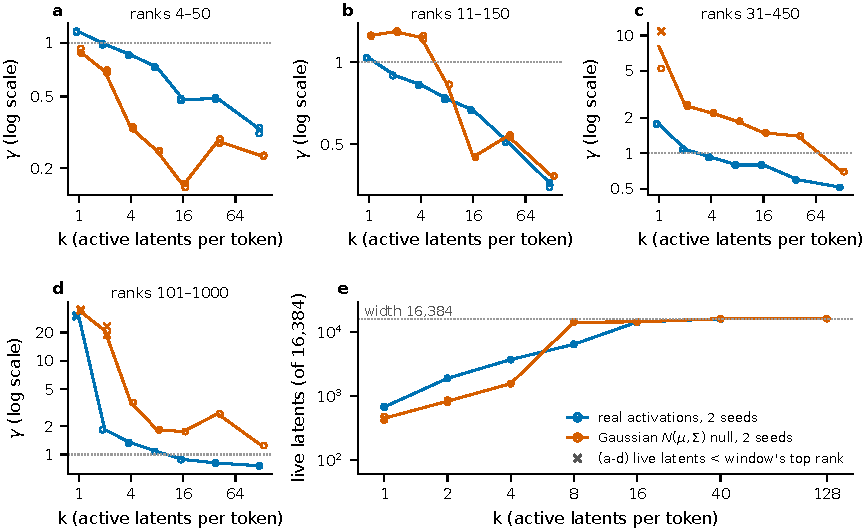
\includegraphics[width=\textwidth]{fig3_gamma_vs_k_L13.pdf}
\caption{$\gamma$ against $k$ at layer 13, width 16,384, for real (blue) and Gaussian-null (orange) SAEs; $\Sig$ from 10M training tokens; live rows. Circles are single seeds (two per point), lines are means, and $\times$ marks a seed with fewer live latents than the window's top rank. In ranks 11--150 the real $\gamma$ falls steadily with $k$. The null's falls in one step between $k=8$ and 16 and is not monotone over $k=16$, 40 and 128, where its range (0.15) is half the real decline (0.31). (e) Live latents against $k$. The Gaussian null keeps 14,400 live latents from $k=8$ up and the real SAE from $k=16$ up; below that the live-count bias of Appendix~\ref{app:live} applies.}
\label{fig:k}
\end{figure*}

The real decoder spectrum flattens steadily with $k$, and the null's flattens in a step (Figure~\ref{fig:k}). In ranks 11--150, over $k=8$--128, the real SAE falls by $0.097$ per doubling and the null by $0.088$, the latter with $R^2=0.61$ because of a drop from 0.826 to 0.448 between $k=8$ and 16. Over $k=16$, 40 and 128 alone, the real SAE falls by 0.103 per doubling (seeds 0.101 and 0.105) and the null by 0.025 (seeds 0.025 and 0.026). We chose this range after seeing the data, because the real SAE has fewer than 6,500 live latents at $k=8$. The null's three values (0.448, 0.536, 0.382) are not monotone. They change by 0.09 and 0.15 between neighbouring $k$, against a seed sd of at most 0.006, so with three points a flat null cannot be told from a slowly declining one. Leaving out one $k$ at a time over $k=8$--128 gives $-0.025$ to $-0.115$ per doubling for the null and $-0.095$ to $-0.103$ for real. In ranks 4--50 over $k=8$--128 the null does not decline ($+0.006$ per doubling, $R^2=0.05$) while real falls by 0.088. In ranks 31--450 the null falls three times faster than real ($0.272$ against $0.092$ per doubling over $k=16$--128).
%% PENDING-GPU: dense k sweep (k = 8, 16, 24, 32, 48, 64, 128) with 3 seeds, decoders kept, scored at a fixed live count. Replace the three-point fits by a condition x log k model with between-k noise, and report it beside the k=8-128 fit.

A sparse control whose dictionary matches Gemma Scope's directions in second moments reproduces the drop in $\gamma$ at small $k$ but only part of the decline above it. We encoded layer-12 activations with the Gemma Scope 65k SAE ($\Lz=72$) and resynthesised training data from its codes, firing each latent independently with its empirical frequency and value distribution. Variant D uses Gemma Scope's decoder rows, randomly re-paired with latents. Variant G uses directions drawn from a Gaussian with the mean and covariance of those rows, so G's dictionary matches Gemma Scope's in its second moments only. Unlike the Gaussian null, G is sparsely codable, and its FVU tracks D's (0.398 against 0.417 at $k=8$, 0.191 against 0.175 at $k=128$). For each of three independent draws of directions and codes we trained 16k TopK SAEs with two seeds at $k=8$, 16, 24, 32, 48, 64 and 128 (84 SAEs) and scored them at a fixed 8,192 live latents (Appendix~\ref{app:resynth}). Before the run we fixed the fit range $k=8$--128 and a rule. G \emph{keeps} D's decline if it retains at least 0.75 of D's per-doubling slope in both $\gamma$ and raw slope, and \emph{removes} it below 0.5 in both, with the window rule of Section~\ref{sec:setup}. In ranks 11--150 G retains 0.78 of D's decline in $\gamma$ and 0.76 in raw slope; paired bootstrap intervals over draws and seeds are $[0.760, 0.798]$ and $[0.748, 0.779]$, so the raw interval reaches just below the threshold. G retains 0.79 in ranks 4--50, 0.62 in ranks 31--450 and 0.53 in ranks 101--1000. All three draws give the same verdict in each window. The pre-registered reading is therefore mixed, with G keeping the decline in the two top windows and part of it in the bulk. Most of the retained decline is the step between $k=8$ and 16, which G reproduces and exceeds ($\gamma$ falls by 0.26 for G and 0.19 for D in ranks 11--150; Figure~\ref{fig:resynth2}). Over $k=16$--128, a range chosen post hoc, G retains 0.45 of D's decline in ranks 11--150 ($[0.43, 0.46]$), 0.13 in ranks 4--50 and 0.53--0.54 in the bulk. Leaving out one $k$ at a time over $k=8$--128 gives 0.45 to 0.88 in ranks 11--150. Second moments of the dictionary, with sparse codes, therefore account for the small-$k$ drop. Much of the steady decline above $k=16$ needs Gemma Scope's own directions, and G's step-then-flatten curve has the shape of the dense Gaussian null's in Figure~\ref{fig:k}.

\section{Cluster structure across layers}
\label{sec:support}

If the mid-stack top window reflects structure beyond $\Sig$, the decoder cloud should cluster more than a covariance-matched cloud does. We clustered the decoder directions of the 16k Gemma Scope SAE nearest $\Lz=70$ at each of the 26 layers (spherical $k$-means, 1,024 and 256 clusters). We did the same for a unit-normalised Gaussian cloud with the decoder cloud's own covariance and count only the excess over it. With 1,024 clusters, the excess between-cluster share of variance and the excess cosine to the cluster centre correlate with the top-window slope at Spearman $\rho=-0.874$ to $-0.910$ (phase-surrogate $p<10^{-4}$). Circular shifts give $p=0.038$, which is the floor for 26 layers. The excess statistics also correlate with $\Sig$'s slope ($\rho=-0.80$ to $-0.82$). Controlling for $\Sig$'s slope leaves partial $\rho=-0.63$ to $-0.78$ (phase $p=0.006$--0.030). Controlling as well for the matched cloud's own clustering leaves $-0.40$ to $-0.58$. In that model the excess cosine stays significant (phase $p=0.009$ and 0.043), and the excess share does not ($p=0.064$ and 0.082). With 256 clusters, $\rho=-0.79$ to $-0.90$, but one cell (excess share, ranks 4--50) has shift $p=0.31$. Two of the four cells fall below the pre-stated survival rule after controlling for $\Sig$ (partial $\rho=-0.64$, $p=0.069$; $-0.57$, $p=0.052$). In the bulk windows $|\rho| \le 0.14$ with 1,024 clusters, but $\rho=-0.42$ and $-0.45$ (not significant) for the excess share with 256. The cluster excess tracks the top-window profile beyond what $\Sig$'s slope explains, with about half its raw strength once the matched cloud's clustering is also controlled. The analysis uses Gemma Scope decoders at one $\Lz$ and has not been run on our real and null SAEs.
%% PENDING-GPU: sparse covariance-matched null and 8-layer real/Gaussian runs. If decoders are kept, run the cluster-excess analysis on real vs null decoders at the same layers; add one sentence here.

Three other candidate sources of the anisotropy have no measurable effect in direct tests (Appendix~\ref{app:fail}). Merging latent pairs with cosine above 0.5 removes up to 34\% of latents in 22 layer-12 SAEs and moves the slope by at most 0.010. Training at layer 13 without the tokens that carry the top 0.1\% or 1\% of values on the massive-activation dimension \citep{sun2024massive} moves $\gamma$ by at most 0.005. The rank-frequency exponent of latent firing does not track the decoder slope as an allocation account would need. Over the 18 layer-12 SAEs with $\Lz < 270$ its rank correlation with the slope is 0.14 ($p=0.59$), and its trends with $\Lz$ within each width are small and of mixed sign ($-0.043$ to $+0.009$ per doubling). It steepens at $\Lz \ge 270$, where the decoder slope is flattest.

\section{Discussion}
\label{sec:disc}

\textbf{Reading decoder spectra.} A decoder slope means little without its $\Lz$, its rank window and a null. At one layer, a doubling of $\Lz$ moves the top-window slope by about 0.1, and a TopK SAE trained only on Gemma's $\Sig$ produces a top-window slope of the same order as the real one. Against that dense null, at $k=40$ and three layers, the real spectrum differs in the bulk and in the layer profile of its top window. The present evidence leaves two questions open. One is how much of each difference comes from sparse codability rather than from structure beyond $\Sig$. The other is whether the profile holds at more than three layers. A sparse dictionary matched to Gemma Scope's directions in second moments reproduces the small-$k$ drop of $\gamma$, so we do not count that drop as a real-data signature. Above $k=16$, a range chosen post hoc, it reproduces 0.13--0.45 of the top-window decline and about half of the bulk decline, which points to a $k$ dependence that needs Gemma Scope's directions beyond their covariance.

\textbf{What the null does.} On Gaussian data a TopK SAE keeps its dictionary close to $\Sig$'s axes and lets variance fall along them much faster than $\Sig$ does. It does not do this by duplicating latents. Real activations hold the dictionary further from $\Sig$'s axes and the bulk flatter. A Gaussian cannot be coded sparsely, which may explain this behaviour. A sparse null with covariance $\Sig$, compared at matched FVU, would show whether the real bulk and profile need more than sparsity plus $\Sig$. Planted-feature generators with $\Sig$'s slope matched, with or without clusters, did not reproduce Gemma's $\gamma(k)$ (Appendix~\ref{app:fail}).

\textbf{Limitations.} The causal comparisons are on one model (Gemma-2-2B) at three layers and one $k$, against a null that cannot be coded sparsely. In Pythia-70m at one layer only the bulk difference and the ranks 4--50 agreement replicate. The $k$ sweep covers one layer, one width and two seeds. The resynthesis control covers one layer and one width (three draws, two seeds), and its codes fire independently. Our TopK slopes use live rows and Gemma Scope's use all rows. The two differ little where nearly all latents are live. That excludes the real $k \le 8$ runs (60--96\% of rows dead) and the null's $k \le 4$ runs (90--97\%), and leaves an uncertainty of about 0.025 at $k=16$ and at the null's $k=8$ (11--12\% dead). The live-count corrections in Appendix~\ref{app:live} assume a Gaussian $\Sig^{\gamma}$ cloud, which real decoders only approximate. Our 65k SAEs drift with width more than Gemma Scope's do. Real $\gamma$ in ranks 11--150 at layer 13 falls from 0.508 at 16k to 0.387 at 65k, which suggests undertraining. The real data were 9.5M tokens seen three times, and the Gaussian samples were fresh. $\Sig$ for Gemma Scope comes from Pile tokens rather than Gemma Scope's training mixture. The scrambled null's steep layer-23 top window ($-0.976$) is unexplained. Cross-layer correlations rest on effective sample sizes of 5 to 10. Against the pre-registered rule of the primary window plus two others, the $\Sig$-decoder correlation of Section~\ref{sec:l0} passes at $\Lz=40$ (ranks 4--50, 11--150 and 31--450) and falls just short at $\Lz=70$ ($p=0.051$ and 0.058 in ranks 31--450). The real-minus-null profile of Section~\ref{sec:profile} is most negative at layer 13 in every top-window cell. In the bulk the difference is smallest at layer 13 in three of four cells and tied in the fourth, but the ratio is not, so it holds in all windows in one unit only. The cluster-excess correlation of Section~\ref{sec:support} holds only in the two top windows, which share most of their ranks, and does not meet the rule.

\section{Conclusion}

Against a Gaussian null with the activations' covariance, at fixed $k$, real activations leave a decoder spectrum with a much flatter bulk and a top window that is steepest, relative to the null, at layer 13 of three layers tested. The top-window magnitude agrees with the null only at some $k$. A sparse dictionary matched to Gemma Scope's directions in second moments reproduces the drop of $\gamma$ at small $k$ but not all of the steady decline above $k=16$. The open question is whether the bulk and profile differences survive a null that is sparse as well as covariance-matched.

\section*{Impact Statement}

This paper concerns how geometric statistics of SAE dictionaries are measured and compared. It recommends reporting such statistics with their sparsity, rank window and a matched null. Without these, a statistic that an SAE would produce from second moments alone can be read as evidence about a model's internal structure. We see no direct route from this work to harm. All models, SAEs and text are public.

\bibliographystyle{icml2026}
\bibliography{thesisA}

\appendix
\onecolumn

\section{Methods}
\label{app:methods}

\textbf{Data and activations.} Gemma-2-2B residual stream after each block (\texttt{resid\_post}), on the uncopyrighted subset of the Pile, context 1,024, beginning-of-sequence position dropped. Pythia-70m layer 3 used context 256. For our Gemma SAEs we cached 10M tokens per layer and held out the last 0.5M for evaluation; $\mu$ and $\Sig$ for the Gaussian null and for $\gamma$ in Tables~\ref{tab:null} and \ref{tab:65k} and Figures~\ref{fig:null} and \ref{fig:k} come from this cache. Figure~\ref{fig:l0}, Section~\ref{sec:l0} and Appendix~\ref{app:li} use the 1M-token $\Sig$.

\textbf{Rank windows in code.} Windows are stored as 0-based slices of the sorted eigenvalues: \texttt{(3, 50)}, \texttt{(10, 150)}, \texttt{(30, 450)} and \texttt{(100, 1000)} are ranks 4--50, 11--150, 31--450 and 101--1000; \texttt{(0, 100)} is ranks 1--100.

\textbf{Our SAEs.} TopK SAEs with an auxiliary TopK loss on dead latents ($k_{\mathrm{aux}}=512$, coefficient $1/32$, a latent is dead after 2M tokens without firing), unit-norm decoder rows with the parallel gradient component removed, Adam with learning rate $2\times10^{-4}\sqrt{16384/n}$ for width $n$ and linear decay over the last 20\% of steps, batch 4,096 tokens, inputs scaled so that $\mathbb{E}\|x\|^2=d$ with the same constant for every condition. Gaussian samples are drawn fresh for every batch (28.5M distinct samples); real data are 9.5M tokens seen three times. Scrambled data permute each coordinate independently across tokens. Seed-to-seed sd at $k=40$ is at most 0.013 in raw slope over all cells of Tables~\ref{tab:null} and \ref{tab:65k} (0.009 for real and Gaussian), and 0.010 for the two $k$-sweep seeds. FVU is measured on the 0.5M held-out tokens.

\textbf{Local SAEs.} The Pythia-70m SAEs of Sections~\ref{sec:top} and \ref{sec:regime} (layer 3, $k=32$, widths 1,024, 4,096 and 16,384, three seeds each for real, Gaussian and scrambled data) make one pass over 15M tokens and are evaluated on 1M further tokens; their $\Sig$ comes from the 20M-token activation cache they are drawn from. The Gemma-2-2B width-4096 $k=40$ SAEs of Section~\ref{sec:regime} are trained on 0.8M tokens at layer 12 (real and Gaussian, $\Sig$ from the 1M-token cache) and on 3M Gaussian samples at layers 0, 3, 7, 13, 17, 21 and 24 ($\Sig$ from 200,508 tokens), and evaluated on 0.2M tokens. The same optimiser settings apply.

\textbf{Gemma Scope SAEs.} Decoder rows of the 288 \texttt{gemma-scope-2b-pt-res} SAEs (all 26 layers at widths 16k and 65k, plus layer 12 at 32k, 131k, 262k, 524k and 1M), all rows, unit norm. Our reproduction of \citet{li2025geometry} (65k SAEs at layers 0, 12 and 24) gives $-0.2383$, $-0.4684$ and $-0.2545$, within 0.02\% of their values; centring and row normalisation change the slope by at most 0.0008. The matched-$\Lz$ layer profiles interpolate each layer's slope linearly in $\log \Lz$ between the two SAEs that bracket the target.

\textbf{Correlations across layers.} Effective sample size from Bartlett's formula with lags up to $n/4$, a Fisher-$z$ interval at that size, 10,000 phase-randomised surrogates of the decoder series, and all 25 circular shifts (resolution $1/26$). We quote the effective-size interval as the conservative one. Partial correlations in Section~\ref{sec:support} are Spearman, with the same surrogates.

\textbf{$\Sig$ estimation.} At layer 12, two halves of the 1M-token sample split by document give slopes within 0.003 of each other in every window. The first 200k tokens alone give bulk slopes steeper by 0.08 (ranks 31--450) and 0.12 (ranks 101--1000), so we use 1M tokens for every Gemma Scope $\Sig$. We have checked convergence at layer 12 only.

\section{Live-count bias}
\label{app:live}

We simulated unit-normalised Gaussian clouds whose covariance is $\Sig_{13}^{g}$ ($\Sig$ at layer 13 raised to a true exponent $g$), with $n$ points, six draws each (sd $\le 0.01$), and measured $\gamma$ in ranks 11--150 (Table~\ref{tab:live}). A finite cloud pulls high $\gamma$ down and pushes $\gamma$ near zero up. Inverting this calibration at each SAE's live count (grid step 0.2, two draws) gives model-based corrected values: the real $k=1$ value moves from 1.034 (672 live latents) to 1.25, the real fit over $k=1$--128 from $1.016-0.094\log_2 k$ to $1.180-0.115\log_2 k$, and the null at $k \le 4$ to 1.36--1.47. These corrections assume a Gaussian cloud with covariance a power of $\Sig$. Real decoder clouds only approximate one (Appendix~\ref{app:matrix}), and the null's decoders are closer to one than real decoders are (Section~\ref{sec:regime}). We do not use the corrected values for any claim in the main text.

\begin{table}[h]
\centering
\caption{Measured $\gamma$ (ranks 11--150) of simulated clouds with true exponent $g$ and $n$ points, $d=2{,}304$.}
\label{tab:live}
\small
\begin{tabular}{l rrrrr}
\toprule
true $g$ & $n=672$ & 2,000 & 4,786 & 8,192 & 16,384 \\
\midrule
0 & 0.183 & 0.123 & 0.089 & 0.071 & 0.054 \\
0.5 & 0.289 & 0.319 & 0.376 & 0.414 & 0.450 \\
1.0 & 0.741 & 0.861 & 0.928 & 0.953 & 0.974 \\
1.25 & 1.027 & 1.137 & 1.192 & 1.213 & 1.228 \\
\bottomrule
\end{tabular}
\end{table}

\section{Width 65,536 and the scrambled null}
\label{app:65k}

\begin{table}[h]
\centering
\caption{As Table~\ref{tab:null}, at width 65,536 (mean of three seeds). FVU and live counts are in Table~\ref{tab:fvu}.}
\label{tab:65k}
\small
\setlength{\tabcolsep}{3.6pt}
\begin{tabular}{l rrr rrr rrr rrr}
\toprule
 & \multicolumn{3}{c}{ranks 4--50} & \multicolumn{3}{c}{ranks 11--150} & \multicolumn{3}{c}{ranks 31--450} & \multicolumn{3}{c}{ranks 101--1000} \\
\cmidrule(lr){2-4}\cmidrule(lr){5-7}\cmidrule(lr){8-10}\cmidrule(lr){11-13}
layer & 3 & 13 & 23 & 3 & 13 & 23 & 3 & 13 & 23 & 3 & 13 & 23 \\
\midrule
real & $-0.218$ & $-0.286$ & $-0.302$ & $-0.246$ & $-0.366$ & $-0.236$ & $-0.420$ & $-0.367$ & $-0.204$ & $-0.515$ & $-0.413$ & $-0.273$ \\
Gaussian $N(\mu,\Sig)$ & $-0.218$ & $-0.228$ & $-0.280$ & $-0.380$ & $-0.460$ & $-0.497$ & $-0.915$ & $-0.861$ & $-0.875$ & $-1.481$ & $-1.176$ & $-1.167$ \\
scrambled & $-0.211$ & $-0.344$ & $-0.403$ & $-0.331$ & $-0.650$ & $-0.967$ & $-1.053$ & $-0.753$ & $-0.700$ & $-1.517$ & $-0.762$ & $-0.240$ \\
\bottomrule
\end{tabular}
\end{table}

The scrambled null's covariance is $\mathrm{diag}(\Sig)$. Its slopes at layers 3, 13 and 23 are $-0.545$, $-1.166$ and $-0.905$ in ranks 11--150 and $-0.976$, $-0.453$ and $-0.126$ in ranks 101--1000. The flat layer-23 bulk of the scrambled SAE, flatter than real at both widths, follows from the flat $\mathrm{diag}(\Sig)$ there. Its steep layer-23 top window ($-0.976$ at 16k) does not follow from a small denominator, since $\mathrm{diag}(\Sig)$ is steeper there than $\Sig$. The median excess kurtosis of the high-variance coordinates is lowest at layer 23 (0.12, against 0.17 at layer 13 and 0.42 at layer 3), so heavy tails do not explain it either.

\section{The bulk as a matrix law}
\label{app:matrix}

\begin{figure}[h]
\centering
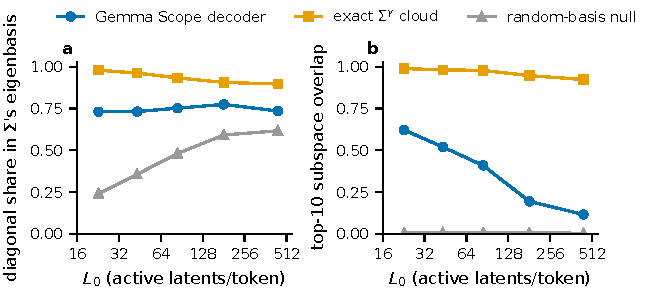
\includegraphics[width=0.62\textwidth]{fig5_matrix_test_1m.pdf}
\caption{Matrix test on the five layer-12 Gemma Scope 16k SAEs ($\Sig$ from 1M tokens). (a) Share of the decoder covariance on the diagonal of $\Sig$'s eigenbasis: real decoders 0.73--0.77 at every $\Lz$, between an exact $\Sig^{\gamma}$ cloud of the same size (0.90--0.98) and the decoder's own eigenvalues in a random basis (0.24--0.62). (b) Overlap of the decoder's and $\Sig$'s top-10 eigen-subspaces, falling from 0.62 at $\Lz=22$ to 0.12 at $\Lz=445$, against 0.92--0.99 for the exact cloud.}
\label{fig:matrix}
\end{figure}

We rotate the decoder covariance into $\Sig$'s eigenbasis, regress its log diagonal on $\log\lambda^{\Sig}$, and compare with two synthetic clouds of 16,384 unit rows (Figure~\ref{fig:matrix}). Over ranks 101--1000 the regression has $R^2=0.955$--0.989 at every $\Lz$ and gives exponents from 0.81 ($\Lz=22$) to 0.37 ($\Lz=445$). In ranks 11--150 it holds only at low $\Lz$ ($R^2 = 0.94$--0.98 up to $\Lz=82$, 0.73 at 176 and 0.01 at 445); at high $\Lz$ the top of the decoder spectrum stops following $\Sig$'s leading directions. Placing each decoder's own eigenvalues in a random basis gives $R^2 \le 0.003$ over ranks 101--1000 and $\le 0.012$ in any window. The same test on local null decoders is in Section~\ref{sec:regime}.

\section{Resynthesis}
\label{app:resynth}

\begin{figure}[h]
\centering
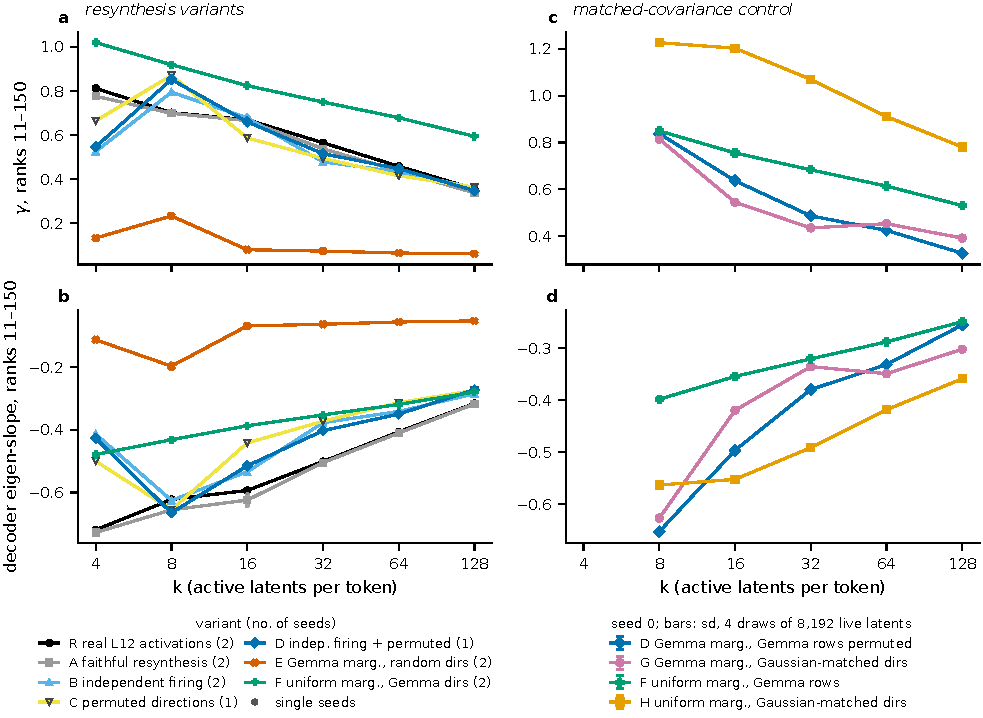
\includegraphics[width=0.85\textwidth]{fig6_resynthesis.pdf}
\caption{Resynthesis at layer 12, ranks 11--150. Left: variants R (real activations), A (faithful resynthesis from codes), B (independent firing), C (permuted decoder rows), D (B and C), E (random directions), F (uniform firing on Gemma Scope's rows); $\gamma$ (a) and raw slope (b). Right: the matched-covariance control at a fixed 8,192 live latents for one draw and one seed (bars: sd over four draws of live latents); Figure~\ref{fig:resynth2} has all three draws and both seeds.}
\label{fig:resynth}
\end{figure}

Source: Gemma-2-2B layer 12, codes from the Gemma Scope 65k JumpReLU SAE. Each variant breaks one ingredient of the resynthesis (Figure~\ref{fig:resynth}). The faithful resynthesis A keeps the real $\gamma(k)$ (per-doubling $-0.095$ over $k=8$--128, against $-0.090$ for real activations). Variants that keep Gemma Scope's directions or their pairing with frequencies keep the decline ($-0.111$ to $-0.122$; C and D one seed). Random directions (E) give $-0.036$, from a curve at the isotropic floor. Uniform firing on Gemma Scope's rows (F) gives $-0.080$ in $\gamma$ but only $-0.037$ in raw slope; F's covariance is the dictionary's own, whose slope ($-0.469$) is the decoder slope of the source SAE, so F is close to circular. The control variant H (uniform firing on Gaussian-matched directions) starts above $\gamma=1$ and recovers little (FVU 0.67 at $k=8$, against 0.50 for F).

\begin{figure}[h]
\centering
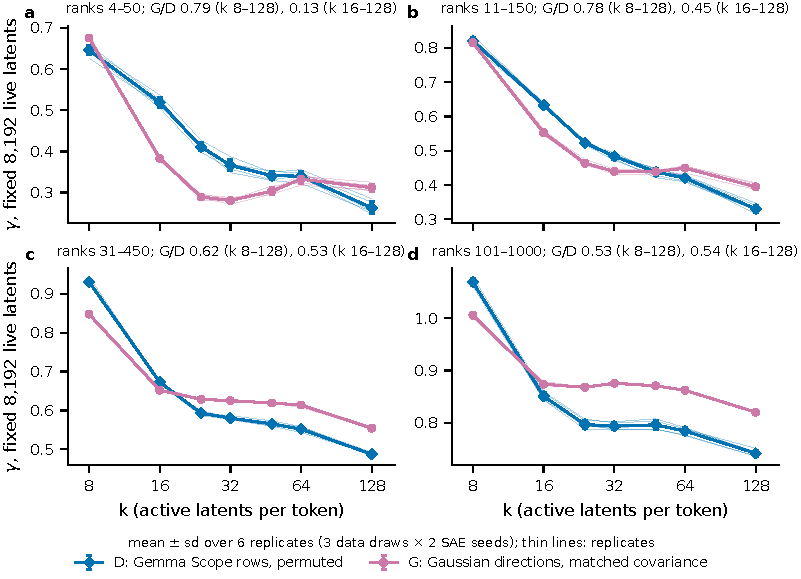
\includegraphics[width=0.8\textwidth]{fig7_resynth_r2.pdf}
\caption{Control G against D at layer 12, width 16,384, in the four rank windows: $\gamma$ at a fixed 8,192 live latents, mean $\pm$ sd over six replicates (three draws of directions and codes, two SAE seeds each); thin lines are single replicates. G follows D's drop between $k=8$ and 16 and then flattens, most clearly in ranks 4--50, while D keeps falling. Panel titles give G's retention of D's per-doubling slope over $k=8$--128 (pre-registered) and $k=16$--128 (post hoc).}
\label{fig:resynth2}
\end{figure}

\begin{table}[h]
\centering
\caption{Control G against D: per-doubling slope of $\gamma$ in $k$ for each variant (mean $\pm$ sd over six replicates) and G's retention of D's slope, in $\gamma$ and raw slope, with paired two-level bootstrap 95\% intervals (draws, then seeds within draws; 20,000 resamples). The verdict uses the fixed-$n$ columns: keeps at $\ge 0.75$ in both units, removes below 0.5 in both. Full-live-count retention is reported only.}
\label{tab:resynth2}
\small
% generated by paper/figures/make_fig_resynth_r2.py from results/r2/resynth_analysis.json
\begin{tabular}{l rr ll rr l}
\toprule
 & \multicolumn{4}{c}{fixed 8,192 live latents} & \multicolumn{2}{c}{full live count} & \\
\cmidrule(lr){2-5}\cmidrule(lr){6-7}
ranks & $s_D$ ($\gamma$) & $s_G$ ($\gamma$) & G/D $\gamma$ [95\%] & G/D raw [95\%] & G/D $\gamma$ & G/D raw & verdict \\
\midrule
\multicolumn{8}{l}{\emph{$k=8$--128 (pre-registered)}} \\
4--50 & $-0.094 \pm 0.002$ & $-0.074 \pm 0.002$ & 0.79 [0.777, 0.810] & 0.79 [0.776, 0.799] & 0.80 & 0.80 & keeps \\
11--150 & $-0.118 \pm 0.004$ & $-0.092 \pm 0.001$ & 0.78 [0.760, 0.798] & 0.76 [0.748, 0.779] & 0.79 & 0.78 & keeps \\
31--450 & $-0.098 \pm 0.001$ & $-0.060 \pm 0.001$ & 0.62 [0.605, 0.624] & 0.62 [0.608, 0.628] & 0.61 & 0.62 & partial \\
101--1000 & $-0.069 \pm 0.001$ & $-0.036 \pm 0.001$ & 0.53 [0.520, 0.533] & 0.54 [0.531, 0.553] & 0.52 & 0.54 & partial \\
\multicolumn{8}{l}{\emph{$k=16$--128 (post hoc)}} \\
4--50 & $-0.076 \pm 0.002$ & $-0.010 \pm 0.003$ & 0.13 [0.104, 0.164] & 0.13 [0.104, 0.161] & 0.11 & 0.11 & removes \\
11--150 & $-0.093 \pm 0.004$ & $-0.042 \pm 0.002$ & 0.45 [0.432, 0.457] & 0.44 [0.423, 0.449] & 0.46 & 0.45 & removes \\
31--450 & $-0.054 \pm 0.001$ & $-0.029 \pm 0.001$ & 0.53 [0.513, 0.542] & 0.53 [0.517, 0.544] & 0.52 & 0.52 & partial \\
101--1000 & $-0.030 \pm 0.001$ & $-0.016 \pm 0.001$ & 0.54 [0.518, 0.557] & 0.55 [0.532, 0.575] & 0.52 & 0.53 & partial \\
\bottomrule
\end{tabular}

\end{table}

The control G against D was pre-registered with the fit range $k=8$--128, the thresholds 0.75 (keeps) and 0.5 (removes) applied to the mean slope over draws, and the window rule. Each draw of directions and codes is independent, and at a given draw D and G share the same code draws, so the comparison is paired. The firing frequencies and 64-quantile value distributions come from Gemma Scope's codes on the first 4M real layer-12 training tokens. Each synthetic dataset has 12M tokens, of which the last 0.5M are held out, and each SAE makes three passes over the other 11.5M. $\gamma$ for each SAE uses the $\Sig$ of its own synthetic dataset, estimated from its 12M tokens. Table~\ref{tab:resynth2} gives the result. Over $k=8$--128 G keeps D's decline in ranks 4--50 and 11--150 and is between the thresholds in both bulk windows, so the pre-registered reading is mixed. The per-draw retention in ranks 11--150 runs from 0.76 to 0.80 in $\gamma$ and from 0.75 to 0.78 in raw slope, and every draw gives the same verdict as the mean in every window. Scoring at the full live count changes no retention by more than 0.02. Over $k=16$--128 (post hoc) G removes the decline in both top windows and is between the thresholds in the bulk. In ranks 11--150 G's mean $\gamma$ at $k=8$, 16, 24, 32, 48, 64 and 128 is 0.815, 0.553, 0.464, 0.440, 0.439, 0.449 and 0.395, and D's is 0.820, 0.633, 0.523, 0.484, 0.438, 0.420 and 0.330 (sd over replicates at most 0.011). $\Sig$'s slope in ranks 11--150 is $-0.77$ to $-0.79$ for every resynthesised dataset. At the first draw and seed, D reproduces the single-draw run of Figure~\ref{fig:resynth} exactly and G within 0.007 in $\gamma$.

\clearpage

\section{Explanations that fail, and planted data}
\label{app:fail}

\textbf{Feature splitting.} If near-parallel latents acted as large spikes, removing them would flatten the spectrum. We greedily merged latents with cosine above 0.5 in 22 layer-12 Gemma Scope SAEs. This removed up to 34.5\% of latents (131k, $\Lz=12$) and changed the ranks 11--150 slope by at most 0.010.

\textbf{Massive activations.} One residual dimension carries rare, very large values. Training our layer-13 16k $k=40$ SAEs (three seeds) without the tokens carrying its top 0.1\% or 1\% of values changed $\gamma$ by at most 0.0052 (ranks 4--50) and at most 0.0017 in the other windows. This test was run at one layer only.

\textbf{Latent-frequency allocation.} \citet{michaud2025manifolds} derive an exponent for the number of latents allocated per feature. If decoder eigenvalues scaled with the number of latents per feature, which is our assumption and not theirs, the eigen-slope would inherit that exponent and would move with $\Lz$ through the frequency distribution. Across 22 layer-12 SAEs the rank-frequency exponent of latent firing (ranks 10 to the last live latent) runs from $-0.59$ to $-0.91$ for $\Lz < 270$ and steepens to $-0.93$ to $-1.01$ at $\Lz \ge 270$, where the decoder slope is flattest. For the 18 SAEs with $\Lz < 270$ the pooled rank correlation with $\Lz$ is 0.13, and within width the trend per doubling of $\Lz$ is $-0.004$ (16k), $+0.009$ (32k), $-0.012$ (65k) and $-0.043$ (131k). Over all 22 SAEs the exponent's rank correlation with the decoder slope in ranks 11--150 is $-0.37$ ($p=0.09$), and 0.14 ($p=0.59$) for $\Lz < 270$. Latent frequencies are not feature frequencies, so this leaves the allocation account underdetermined.

\textbf{Planted features.} Synthetic activations built as sparse sums of planted features at $d=2{,}304$, with $\Sig$'s slope matched to Gemma's in every window, did not reproduce Gemma's $\gamma(k)$ in ranks 11--150. The best root-mean-square distance to Gemma's curve was 0.27 without clusters and 0.24 with planted clusters of 16 features at cosine 0.6 to a centre, against a pre-registered pass test of RMS below 0.15 and a per-doubling slope within 0.04 of Gemma's. Over $k=4$--128 every planted curve was nearly flat ($-0.009$ to $+0.018$ per doubling for seven generators, against $-0.095$ for Gemma over the same range). Five of the seven generators ran one seed and two ran two. The generator with 4,608 features has a jagged curve and gives $-0.074$ over $k=8$--128. A point-feature generator whose $\Sig$ was not slope-matched (it has a plateau over its top eigenvalues) came within RMS 0.14 of Gemma's curve on one seed, but its $\gamma$ falls by only 0.041 per doubling over $k=4$--128 and fails the slope part of that test.

\section{Activation spectra under other protocols}
\label{app:li}

\begin{table}[h]
\centering
\caption{Layer 12, 1M tokens: eigen-slope of the activation spectrum under five preprocessing choices, against the decoder of \citeauthor{li2025geometry}'s SAE (65k, $\Lz=72$ by release name, 75.8 measured).}
\label{tab:li}
\small
\begin{tabular}{l rrrr}
\toprule
 & ranks 1--100 & 11--150 & 31--450 & 101--1000 \\
\midrule
decoder cloud (centred) & $-0.462$ & $-0.468$ & $-0.418$ & $-0.503$ \\
activations, raw, centred ($\Sig$) & $-0.923$ & $-0.883$ & $-0.732$ & $-0.717$ \\
activations, raw, uncentred & $-1.031$ & $-0.902$ & $-0.739$ & $-0.718$ \\
activations, unit-norm tokens, centred & $-0.880$ & $-0.864$ & $-0.748$ & $-0.731$ \\
activations, unit-norm tokens, uncentred & $-1.012$ & $-0.881$ & $-0.753$ & $-0.732$ \\
activations, per-dimension standardised & $-0.446$ & $-0.489$ & $-0.535$ & $-0.600$ \\
\bottomrule
\end{tabular}
\end{table}

Table~\ref{tab:li} gives the layer-12 grid. With fewer tokens the raw spectrum flattens (ranks 1--100: $-0.63$ at 256 tokens, $-0.78$ at 1,024, $-0.91$ at 16,384) but stays steeper than the decoder. Reading ``activations'' as the SAE's codes gives $-0.987$ (ranks 1--100).

At all 26 layers, on the 1M-token covariance, we compared the activation spectrum with two decoders: Li et al.'s 65k SAE at each layer, and the 16k SAE whose $\Lz$ is nearest 40. Under the raw centred and raw uncentred covariance the activation spectrum is steeper than both decoders at 26 of 26 layers in ranks 1--100 and 11--150 ($\gamma$ 0.24--0.60). Under the correlation matrix, Li et al.'s ordering holds in ranks 1--100 at layers 11--14 against their SAEs (4 of 26; 2 of 26 in ranks 11--150) and at layers 10--18 against the 16k SAEs (9 of 26; 8 of 26 in ranks 11--150), with $\gamma$ up to 1.15 and 1.28. The correlation-matrix spectrum is the most sensitive to sample size: at layer 12 it is $-0.544$ on 32,736 tokens and $-0.446$ on 1M. We could not test other models, hooks or text distributions.

\end{document}
